\documentclass[12pt]{article}
\usepackage[utf8]{inputenc}
\usepackage[spanish]{babel}

\usepackage[left=2.5cm, right=2cm, top=2.5cm, bottom=2cm]{geometry}

\usepackage{helvet}
\renewcommand{\familydefault}{\sfdefault}
\usepackage{graphicx}
\usepackage{float}

% Title Page
\title{El software libre en el ámbito espacial}
\author{Arias Emmanuel}
\date{5 de noviembre de 2018}


\begin{document}
\maketitle
\newpage

\begin{abstract}
	El desarrollo de proyectos satelitales conlleva costos que son de importante magnitud. A estos los se los puede clasificar en cinco grandes categorías: a) desarrollo (propiamente dicho), b) materiales, c) ensamblado, integración y tests, d) lanzamiento y e) operaciones. La mayor parte de los costos se lo llevan los componentes que se utilizan para desarrollar un satélite, debido a que estos componentes son especiales, ya que están ''calificados para volar''. 
	
	El desarrollo también cubre una parte importante de los costos, siendo el software participe de este porcentaje. Por lo tanto, para lograr reducir el costo de los proyectos satelitales es importante, la utilización de software libre y/u open source ya que de esta manera va a permitir evitar licencias costosas. Además, lo más importante es que se tiene un total control y conocimiento del código que se está ejecutando, teniendo la libertad de poder modificarlo, para así de esta manera moldear el software al proyecto que se está encarando.
	
	A lo largo de este trabajo se presenta la definición de Software libre y Open source, y se presentan una serie de ejemplos de software que es utilizado comúnmente en el ambiente espacial. 
\end{abstract}

\section{Software libre}
La definición de software libre presenta los criterios para decidir si un software en particular califica como libre. Tal como se indica en \cite{freesw}, el ''open source'' es una filosofía muy diferente al SL y se encuentra basado en diferentes valores. 

Como  ya es sabido el SL, se basa en cuatro libertades:
\begin{itemize}
	\item \textbf{Libertad 0}: Es la libertad de ejecutar un programa como se desee, y para cualquier propósito.
	\item \textbf{Libertad 1}: Es la libertad de estudiar cómo funciona un programa, y realizar modificaciones. Para ello es necesario poder acceder al código fuente. 
	\item \textbf{Libertad 2}: Es la libertad de redistribuir copias, con esto, se puede ayudar a las demás personas. 
	\item \textbf{Libertad 3}: Es la libertad de distribuir copias de versiones modificadas del software original. Con esto se le brinda a la comunidad la oportunidad de beneficiarse por los cambios realizados en el software. 
\end{itemize}

Si un software cumple con estas libertades, se puede indicar que este software es ''libre'', en caso contrario es clasificado como ''non-free''.

''Free software'' no significa ''software no comercial''. Un SL puede ser de uso comercial, nada lo impide \cite{freesw}. Por ejemplo, Red Hat es una empresa multinacional que provee SL a empresas. Red Hat crea, mantiene y contribuye a una gran cantidad de proyectos de SL, además adquirió software propietario y ha liberado el código. 

En inglés, surge el problema de que Free Software se confunde con software gratuito, ya que ''free'' tiene el doble significado de ''libre'' y ''gratis''. Esto no sucede en el español, ya que existe una palabra diferente para el concepto de libre y gratis. Pero vale aclarar que SL no es igual a gratuito. 


\section{Open Source}
El movimiento del software libre nace en 1983 de la mano de Richard Stallman, el cual lanza en ese año el \textit{GNU Project}. Luego, en 1985 Stallman crea la \textit{Free Software Foundation}. Tal como lo explica Stallman en \cite{richard-open}, SL no es lo mismo que Open Source. En 1998 una parte de la comunidad del SL se separa del movimiento, y crea lo que denominaron ''open source''. Este término fue adoptado para evitar un posible mal entendimiento de la palabra SL, pero tiene puntos de vistas diferentes al movimiento.  

Si bien, los dos términos describen casi la misma categoría de software, el open source se refiere a una metodología de desarrollo, se preocupa sobre como hacer mejor el software (solo en el sentido práctico). Mientras que el SL es un movimiento social \cite{richard-open}, un compromiso ético que respeta las libertades de los usuarios de software. 

Todo SL clasifica como open source, pero en contraposición, no todo open source clasifica como SL, ya que existen muchas licencias que van en contra de las libertades. 

\section{El costo de los proyectos satelitales}
Toda misión satelital está dividida en 3 grandes segmentos:
\begin{itemize}
	\item Segmento de vuelo
	\item Segmento de tierra
	\item Segmento de usuarios
\end{itemize}

El \textit{segmento de vuelo} es el satélite propiamente dicho. Este, a su vez está dividido en dos partes:
\begin{itemize}
	\item \textbf{Plataforma de servicio}: es el satélite propiamente dicho. Este tiene varios subsistemas, que en forma general son los siguientes (varían de misión a misión):
	\begin{itemize}
		\item \textbf{Command and Data Handling Subsystem}: Es el cerebro del satélite, es la computadora que controla que se ejecuten correctamente los comandos que son enviados, recolecta datos de salud de los diferentes componentes (housekeeping). 
		\item \textbf{Power Subsystem}: Es la parte que se encarga de alimentar eléctricamente todos los componentes. Este incluye las baterías y los paneles solares.
		\item \textbf{Thermal Subsystem}: Es el subsistema que se encarga de controlar la temperatura en satélite. Se debe recordar que en el espacio no hay atmósfera que regule la temperatura, entonces el satélite pasa por varios ciclos de muy altas temperaturas a muy bajas en cuestión de segundos, debido al movimiento de este al rededor de la Tierra. 
		\item \textbf{Communication Subsystem}: Este subsistema se encarga de la comunicación del satélite con las estaciones terrenas. A través de este subsistema se envía la telemetría, recibe comandos, y envía las imágenes o cualquier otra información que tenga el satélite. 
		\item \textbf{Propulsion Subsystem}: Este es el subsistema que se encarga de corregir órbita, realizar maniobras ante eventualidades. Este está conformado principalmente por las toberas que permiten realizar los movimientos. 
		\item \textbf{Attitude and Orbit Control Subsystem}: Este subsistema tiene todos los sensores necesarios para indicarle al satélite (y a los operadores) cómo es la actitud (posición) del satélite.
	\end{itemize}

	\item \textbf{Payload (o carga útil)}: Este está conformado por todos los instrumentos que son necesarios para cumplir con la misión por que da origen a todo. Este incluye cámaras, radares, sensores, etc. 
\end{itemize}

El desarrollo de proyecto satelitales conlleva costos que son de importantes magnitud \cite{Cate-Emma}. Este costo se puede clasificar en 5 grandes categorías:
\begin{itemize}
	\item Desarrollo
	\item Materiales
	\item Ensamblado, integración y test
	\item Lanzamiento
	\item Operaciones
\end{itemize}

De estos, el desarrollo y los materiales se llevan un mayor porcentaje de los costos. Esto es así porque para construir satélites se utilizan componentes que deben estar ''calificados para volar'', esto quiere decir que deben soportar el ambiente hostil del espacio. De otra forma, los componentes fallarían, esto representaría el fin de la misión y por lo tanto la pérdida de millones de dolares. 

El \textit{segmento terreno}, está compuesto por todos los sistemas necesarios para poder comandar al satélite, descargar telemetría, y poder conocer cuál es el estado de salud del satélite, todos los sistemas necesarios para dar seguimiento al mismo, y poder calcular su órbita (en otras palabras, no perder el satélite). Así mismo, aquí es dónde se descargan las imágenes, y se hacen los primeros procesamientos. También se puede indicar que aquí se incluyen las estaciones terrenas, o su gestión si se trata de estaciones terrenas extranjeras.

Por último, tenemos el \textit{segmento de usuario} (o a veces también llamado de ciencia), son todos aquellos que se benefician con las imágenes. Aquí se encuentran todos los sistemas y personas que trabajan con las imágenes para obtener información de estas. Las imágenes pueden ser ''cruzadas'' con otros tipo de datos, para así de esta manera, aumentar el grado de calidad de la información que se obtienen. 

\section{Software libre y/u open source en el área espacial}
Se deja de lado el tratamiento de los altos costos de los materiales (Hardware), que se utilizan, para los ingenieros electrónicos. Este artículo busca concientizar sobre el uso de Software privativo, licenciado y costoso en el ámbito espacial. Esto es aplicable al desarrollo de software de cualquier ámbito: académico (esta debe ser el área promotora del uso del software libre), gubernamental (idem al académico), medicinal, nuclear, militar, etc.  

El uso del open source o SL tiene múltiples ventajas. La principal de ellas es que no se deben pagar licencias costosas para su uso, ni tampoco se queda ligado al uso de una plataforma determinada, lo cual tiene como consecuencia la utilización de sus servicios exclusivos ante cualquier tipo de problema. 

Otra desventaja, del uso de software privativo en industrias que son ''sensibles'', es que no se tiene en cuenta cuál es el verdadero funcionamiento del mismo. Es decir, no se sabe a ciencia cierta qué está haciendo internamente el software durante su ejecución. Esto puedo traer consecuencias desastrosas, si por ejemplo, el código calcula incorrectamente ciertas variables que son vitales para el funcionamiento.

Conocer el código del software que tiene a su cargo el funcionamiento de un sistema que es ''crítico'' es de suma importancia por los motivos mencionados anteriormente. 

Muchas veces, se cae en el error de pensar que no existe un SL u open source que realice las mismas tareas que realiza un software privativo, pero esta es una idea errónea. Si, no hay que negar, muchas veces los software privativos tienen más publicidad o son más ''vistosas'' o user-friendly, pero poco a poco esta tendencia va cambiando. 

\section{Algunos softwares utilizados}
Hay que aclarar, que cada misión satelital tiene sus propias políticas en cuanto al uso y desarrollo de software. La mayoría de las agencias espaciales, no liberan código, debido a razones de seguridad. Pero organizaciones como la NASA tienen varios proyectos de código abierto, que si bien, no forma parte directamente de la operación de sus misiones, son excelentes herramientas que ayudan a otras agencias, y a personas dedicadas a la actividad espacial, ya sea profesionalmente o aficionados. 

Más allá de las políticas de cada organización, esto no quita que las mismas agencias espaciales se beneficien del uso del software no privativo. 

\subsection{Papyrus}
Papyrus\footnote{https://www.eclipse.org/papyrus/} un editor gráfico que pertenece a Eclipse Foundation. Esta es una poderosa herramienta que permite realizar diversos modelos. Es utilizado debido a sus extensos Plugin. Entre los diferentes estándar que maneja, destaca por su soporte a SysML (System Modeling Language).

\begin{figure}[H]
	\centering
	
\includegraphics[width=0.7\linewidth]{papyrus}
	\caption{Logo Papyrus}
	\label{fig:papyrus}
\end{figure}

\begin{figure}[H]
	\centering
	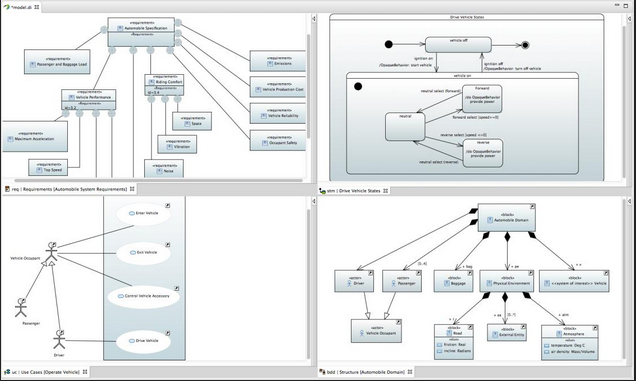
\includegraphics[width=0.7\linewidth]{papyrus2}
	\caption{}
	\label{fig:papyrus2}
\end{figure}

\subsection{Gpredict}
Gpredict\footnote{https://github.com/csete/gpredict} es un software de tracking y predicción de órbita en tiempo real. Este usa los algoritmos SGP4/SDP4 de propagación junto con un conjunto de tle\footnote{two-line element sets} de NORAD\footnote{https://www.noradsanta.org/}. Este software tiene la capacidad de poder cargar las posiciones (latitud y longitud) de las estaciones terrena y sus rangos de visión, de esta manera es posible predecir AOS (Acquisition of Signal) y LOS (Lose of Signal) de los satélites.

\begin{figure}[H]
	\centering
	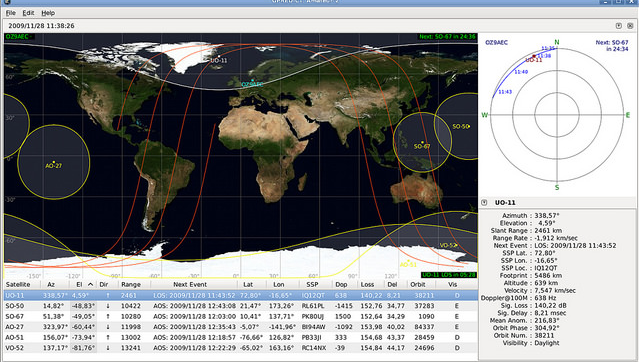
\includegraphics[width=0.7\linewidth]{gpredict}
	\caption{GUI de Gpredict}
	\label{fig:gpredict}
\end{figure}

\subsection{FreeRTOS}
FreeRTOS\footnote{https://www.freertos.org/} es un microkernel de sistema operativo de tiempo real (RTOS). Es utilizado en en sistemas embebidos y tiene aplicación en aproximadamente 35 microcontroladores. 

\begin{figure}[H]
	\centering
	
\includegraphics[width=0.7\linewidth]{freertos}
	\caption{Logo de FreeRTOS}
	\label{fig:freertos}
\end{figure}

\subsection{Distribución de Linux}
Las distribuciones de linux son sistemas operativos que usan el kernel de Linux. Estas distribuciones son gratuitas con esto se evita el pago de costosas licencias. Debe destacarse que en una misión satelital se necesitan una gran cantidad de computadoras (las usadas por cada integrante del proyecto), y además en grandes infraestructuras virtualizadas se exige la existencia de cientos de VMs (virtual machines) las cuales deben funcionar con un sistema operativo. 

\subsection{SOPI}
SOPI\footnote{https://sopi.conae.gov.ar/} es un proyecto de desarrollo de software nacional que es utilizado para el procesamiento de imágenes satelitales. SOPI está diseñado para visualizar, procesar y analizar imágenes de sensores remotos, de acuerdo a las necesidades de los usuarios y a las características de las misiones satelitales\cite{sopi}. Este software compite directamente con softwares de la talla de ENVI cuya licencia es costosa. 

\begin{figure}[H]
	\centering
	
\includegraphics[width=0.7\linewidth]{sopi}
	\caption{Logo de SOPI}
	\label{fig:sopi}
\end{figure}

\subsection{Python}
Python es un lenguaje de programación interpretado de propósito general desarrollado por Guido van Rossum en 1991. Este ha sido creado con el propósito de ser sencillo de a prender y de leer. Tiene un sintaxis y semántica sencilla, que ayudado por la comunidad de desarrolladores a través de la creación de módulos y mejoras en el lenguaje, hacen que Python sea una excelente opción a la hora de realizar software de manera veloz, confiable y portable, esto se debe a que el interprete está disponible para la mayoría de los sistemas operativos actuales. 

\begin{figure}[H]
	\centering
	
\includegraphics[width=0.7\linewidth]{python}
	\caption{Logo Python}
	\label{fig:python}
\end{figure}


Python ha crecido popularmente en los últimos años, debido a las bondades que se mencionan en el párrafo anterior. Según \cite{python-trend} el crecimiento de la tendencia de Python (ver Figura \ref{fig:pythontrend}) se debe al \textit{boom} de la Inteligencia Artificial y el Data Science, sumado a esto, es que es un lenguaje muy simple de aprender. 

\begin{figure}
	\centering
	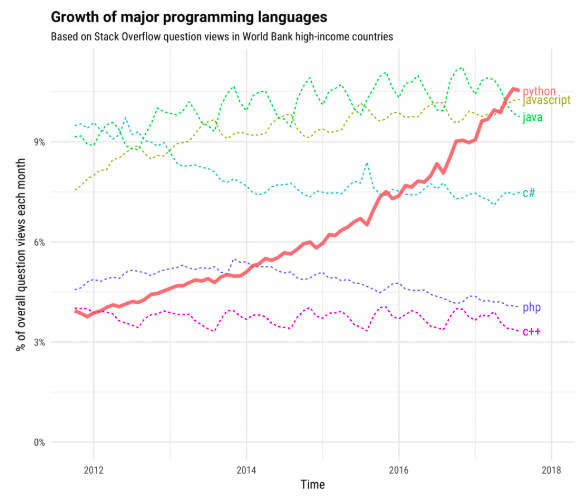
\includegraphics[width=0.7\linewidth]{pythontrend}
	\caption{Tendencia del lenguaje Python. Fuente: \cite{python-trend}}
	\label{fig:pythontrend}
\end{figure}

Python es muy utilizado en el ambiente espacial, basta observar el repositorio de NASA (ver Figura \ref{fig:nasa} )\footnote{https://code.nasa.gov/}\footnote{https://github.com/nasa/} u otros proyectos tales como Sunpy\footnote{https://sunpy.org/} o Astropy\footnote{http://www.astropy.org/}.

\begin{figure}[H]
	\centering
	
\includegraphics[width=0.7\linewidth]{NASA}
	\caption{CODE.NASA.GOV}
	\label{fig:nasa}
\end{figure}

\section{Conclusión}
El software libre y el open source juegan papeles importantes a la hora de encarar cualquier proyecto. La decisión de utilizar software no privativo trae consigo grandes beneficios como evitar el pago del costosas licencias que tiene como principal objetivo quitar las libertades que todo ciudadano podría aspirar. La utilización de software privativo tiene como propósito ligar al proyecto y/u organización a la empresa desarrolladora, eliminando de esta manera toda posibilidad de conocer el funcionamiento del software y de cambiarlo, por parte del consumidor del mismo. 

Por tales motivos, en este trabajo se aconseja, que cada proyecto a encarar, sea del ámbito que sea (en este caso espacial), se utilice software libre, para así de esta manera tener un control estricto del software que se utiliza y si, existiese la posibilidad y las capacidades, poder modificarlo, y optimizar su funcionamiento amoldado al proyecto que se está trabajando.

\newpage

\bibliography{biblio}
\bibliographystyle{abbrv}

\end{document}          
